% This is a simple sample document.  For more complicated documents take a look in the exercise tab. Note that everything that comes after a % symbol is treated as comment and ignored when the code is compiled.

\documentclass{article} % \documentclass{} is the first command in any LaTeX code.  It is used to define what kind of document you are creating such as an article or a book, and begins the document preamble

\usepackage{amsmath} % \usepackage is a command that allows you to add functionality to your LaTeX code
\usepackage[a4paper, margin=1in]{geometry}
\usepackage{mathptmx}
\usepackage[T1]{fontenc}
\usepackage{graphicx}
\usepackage{tabularx}
\usepackage{hyperref}


\title{Simple Sample} % Sets article title
\author{My Name} % Sets authors name
\date{\today} % Sets date for date compiled

% The preamble ends with the command \begin{document}
\begin{document} % All begin commands must be paired with an end command somewhere

\begin{center}
 \Large \textbf{POLITECHNIKA BYDGOSKA} \\
  im. Jana i Jędrzeja Śniadeckich \\
\end{center}

\begin{center}
\end{center}

\begin{center}
 \LARGE WYDZIAŁ TELEKOMUNIKACJI, INFORMATYKI I ELEKTROTECHNIKI \\
\end{center}

\begin{center}
 
\includegraphics[width=4cm,height=4cm]{logo.png}
 % logo.png: 300x300 px, 72dpi, 10.58x10.58 cm, bb=0 0 300 300
\end{center}

\begin{center}
 \Large \textbf{PRACA DYPLOMOWA INŻYNIERSKA}
\end{center}

\begin{center}
 \large \textbf{na kierunku Informatyka Stosowana}
\end{center}

\vspace{3cm}

\begin{center}
 \LARGE \textbf{Interaktywny konfigurator wnętrz pomieszczeń z dekoracyjnymi panelami 3D}
\end{center}

\vspace{3cm}

\begin{minipage}{2in}
Pracę wykonał: \\
Antoni Malak\\
\end{minipage}
\hfill
\begin{minipage}{1.3in}
Kierujący pracą: \\
dr inż. Mariusz Sulima
\end{minipage}


\begin{minipage}{2in}
Nr albumu: \\
108650
\end{minipage}

\begin{center}
 Bydgoszcz,
\end{center}


\newpage

\hspace{0pt}
\vfill

\begin{center}
\Huge Tutaj wstawić kartę pracy
\end{center}

\vfill
\hspace{0pt}

\newpage

\section*{Streszczenie}
Celem pracy jest zaprojektowanie oraz stworzenie interaktywnego konfiguratora elementów wnętrz, a dokładniej ściennych paneli dekoracyjnych. Najpierw opisane będą istniejące już rozwiązania w tym zakresie, a potem zostanie określony zbiór funcjonalności oraz zakres interaktywności. Wymagane będzie zdefiniowanie i wymodelowanie elementów wnętrza, a następnie zaprojektowanie logiki programu umożliwiającej edycję parametrów tychże elementów.
\\

\textbf{Słowa kluczowe:}

\section*{Summary}

\textbf{Keywords:}

\newpage

\tableofcontents

\newpage

\section{Wstęp}

% <okoliczności powstania pracy>
% -dostępność reklamy
% -funkcje wizualizacji

Szybki rozwój oraz powszechnośc internetu pozwolił na łatwiejsze dotarcie do potencjalnego klienta. Podając jedynie adres strony internetowej, zaprosić można kogoś na stronę internetową, której budowa i funkcje mogą być najróżniejsze. Może to być prosta statyczna strona wizytówka, której celem jest reklamowanie kogoś lub czegoś, lub skomplikowany profesjonalny program, który jest dostepny dla każdego, albo coś pomiędzy...
\\

Dawniejszą formą reklamy były bannery reklamowe i ulotki. Bannery zwracały uwagę masy osób, a ulotki pełniły rolę informcyjną, podsuwając klientowi bardziej szczegółowe informacje, dotyczące produktu. Niestety pewne rzeczy lepiej ejst przedstawić w sposób graficzny, dalatego powstały katalogi, w których widać produkt w jego 'naturalnym środowisku'. Dzięki technologii możliwe jest dostarczenie podobnej reklamy poprzez internet, nie marnując przy tym papieru, oraz dając sobie jednocześnie więcej możliwości w postaci interaktywności.
\\

Dzięki zaimplementowaniu funkcji interaktywnych w konfiguratorze, możliwe będzie rozszerzenie zestawu funkcji ze statycznego obrazu do namiatki wizyty w salonie sprzedającym ten produkt. Ważne jest odpowiednie podejście do wizualizacji. Możliwe będzie obejrzenie pojedynczego panelu, ale bardziej pomocny dla klienta będzie widok przykładowego wnętrza, z ich użyciem. Możliwa będzie częściowa edycja panelu, oraz pomieszczenia w którym będzie on przedstawiany.
\\


    \subsection{Cel pracy}
Celem tej pracy dyplomowej jest stworzenie interaktywnej wizualizacji wnętrz, przedstawiającej panele ścienne potencjalnemu klinetowi. Możliwy będzie wybór panelu z katalogu, zmiana jego koloru, oraz definiowanie sposobu ich ułożenia. Możliwa będzie również konfiguracja wnętrza, aby klient mógł obejrzeć produkt, przedstawiony we wnętrzu, które przypomina jego własny dom. Do wyboru będą z góry zdefiniowane pomieszczenia, pozwalające na częściowe dostosowywanie ich w kwestii kolorystyki wnętrza, ilości i rozmiaru okien oraz konfiguracji mebli. Ważnym aspektem będzie możliwość osadzenia programu na stronie internetowej, co zwiększy rzeszę potencjalnych klientów.
\\

Przed napisaniem programu, wymagana będzie analiza podstawowych pojęć związanych z tematem, w celu lepszgo zrozumienia tematu, oraz precyzyjniejszego nakreślenia zakresu funkcji, które powinien pełnić program. Trzeba będzie przeanalizować i porównać istniejące już rozwiązania, aby nowo powstały program nie powielał błędów swoich poprzedników i starał się inspirować ich mocnymi stronami. Warto byłoby rozłożyć ideę na czyniiki pierwsze i zastanowić się nad różnymi ich aspektami, dzieląc te już isteniejące na kategorie i porównując je ze sobą.
\\

Dopiero potem możliwe będzie poprawne zdefiniowanie założeń i zakresu funkcji programu. Wyciągając wnioski z podobnych rozwiązań, będzie można zaprojektować rozwiązanie idealnie pasujące do postawionego problemu. Zdefiniowany zostanie zakres funkcjonalności, które powinna pełnić taka aplikacja. Ważne również będzie uprzednie zdefiniowanie stopnia interaktywności, gdyż implementacja pewnych funkcji nie może być możliwa w późniejszym stadium programowania. Warto również zastanowić sie nad funkcjami jakie powinna pełnić internetowa aplikacja, która pełni również rolę reklamy.
\\

Po fazach analizy i projektowania, możliwe będzie przejście do właściwej implementacji projektu, zaczynając od zaprogramowania logiki programu, poprzez modelowanie obiektów trójwymiarowych, aż do stworzenia wizualizacji, którą będzie można osadzić na stronie internetowej.
\\



\section{Wstęp teoretyczny}
   
    \subsection{Wizualizacja}
        Wizualizacja jest obrazową reprezentacją przedmiotu, procesu lub stanu. Dawniej odnosiło się to do obrazu, albo procesu jego tworzenia, w naszej ludzkiej wyobraźni. Obraz ten istniał jedynie w naszej głowie, by przedstawić go komuś innemu wymagane było nakreślenie jego na jakimś medium, co wymagało dużych umiejętności i środków. Cała gałąź sztuki polega własnie na doskonaleniu tego wymagającego procesu.
        \\
        
        Wizualizacja komputerowa zajmuje się czymś podobnym. Stara się przedstawić coś nie fizycznego za pomocą ilustracji. Przedstawiany może być przedmiot, proces albo inny bardziej abstrakcyjny koncept. Dzięki oprogramownaiu graficznemu możliwe jest zautomatyzowanie tego procesu dla, z góry określonych, scenariuszy. Zadaniem wizualizacji komputerowej jest zebranie ogromu danych, odpowidnie ich przetworzenie, oraz przedstawienie ich w prosty i zrozumiały sposób użytkownikowi końcowemu.
        \\
        
        Medium komputerowe pozwala na wiele możliwości w kwestii edycji prezentowanej grafiki. Parametry mogą zostać łatwo zmienione, a ich zmiana może zostać odzwierciedlona w warstwie graficznej. Mogą się one tyczyć działania całego programu i jego algorytmów, albo części renderującej grafikę. Peryferia komputerowe pozwalają na łatwe wprowadzanie i dostrajanie parametrów, a program bierze te zmienione wartości pod uwagę tworząc nowy, zmieniony obraz. Funkcja pozwalająca na wprowadzanie zmian w symulacji, oraz natychmiastowa jej reakcja jest podstawą interaktywności.
        \\
            
    \subsection{Interaktywność}
        Interakcja jest wzajemnym oddziaływaniem na siebie osób, przedmiotów lub zjawisk.\footnote[1]{Definicja z internetowego słownika PWN} Ważne żeby oddziaływanie te było dwu-kierunkowe, gdyż jednokierunkowym odpowiednikiem interakcji jest przyczynowość. Interaktywność jest miarą interakcji i jej jakości. 
        \\
    
        Interaktywnośc jest sytuacją w której każda kolejna akcja bierze poprzednią, lub kilka porzednich, pod uwagę zmieniając jej kontekst. Wykonanie tej samej akcji w innym kontekście będzie skutkować wykonaniem innej czynności. Ważne jest aby różne konteksty były łatwo rozpoznawalne i znane użytkownikowi.
        \\
    
        Interaktywność może zostać zdefiniowana jako ciągła wymiana informacji, pomiędzy minium dwoma uczestnikami.  W tym przypadku jednym uczestnikiem jest wizualizacja, a drugim użytkownik. Użytkownik podaje informacje w postaci parametrów wejściowych, a wizualizacja zwraca użytkownikowi jak wyglądać może scena spełniające podane wymagania i paramtery. Jest to proces który zachodzi cały czas w formie pętli, lecz nie każda akcja użytkownika musi równać się natychmiastowej reakcji systemu.
        \\
        
        Ważne jest zachowanie przejrzystości po obu stronach. Należy dać użytkownikowi interfejs, który jest zrozmiały i łatwy w obsłudze. Dzięki zastosowaniu się do podstawowych zasad projektowania interfejsów powinien on być wizualnie przejrzysty i jednolity. Sensowne rozplanowanie różnych kontekstów, pozwoli na bardziej intuicyją nawigację po programie i jego funkcjach.
        \\
    
        Interaktywnośc pozwala użytkownikowi na kontrolowanie parametrów wejściowych symualcji, oraz obserwowanie nowo powstałego obrazu. Ważne jest aby użytkownik czuł, że ma kontrolę nad przebiegiem symualcji, a każda wprowadzona zmiana jest wprowadzana i aktualizowana tak szybko jak szybko się da. Dlatego czas obliczenia kolejnego widoku powinien być odpowiednio krótki. Zawęża to częściowo jak wiele obliczeń możemy przeznaczyć na ten cel, oraz jak wymagająca i realistyczna może być wizualizacja i jej grafika. 
        \\
                
    \subsection{Grafika komputerowa}
        Grafika komputerowa jest dziedziną zajmującą się tworzeniem, przetwarzaniem oraz wyświetlaniem obrazów w medium komputerowym. Obraz może być wygenerowany przez komputer, tworząc obraz generowany komputerowo (tzw. CGI), albo może być odzwierciedleniem prawidziwego fizycznego obiektu. Do stworzenia zdjęcia obiektu używane są matryce światłoczułe, zmieniające docierające do niej fotony, na sygnał cyfrowy. Możliwe jest również stworzenie obrazu, będącego wizualizacją powstałą z pomiarów innych urządzeń i sensorów cyfrowych. Mogą to być zarówno wykresy przedstawiające zmianę wartości mierzonej przez sensor, albo coś bliższego obrazowi obiektu jak trójwymiarowy model powstały z zeskanownia bryły fizycznego obiektu.
        \\
        
        Podstawowe biblioteki graficzne, takie jak SDL, OpenGL, pozwalają na rysowanie podstawowych kształtów, obrazów i stosowanie podstawowych przekształceń na tych obrazach. Może to być wystarczające do stworzenia prostych wizualizacji, ale aby osiągnąć oczekiwane wyniki wymagany byłby ogromny wkład pracy. Biblioteki te nie pozwalają na wyświetlanie skompikowaynch modeli trójwymiarowych, ani ich tekstur. Oświetlenie musiałoby być zaimplementowane od podstaw wymagając ogromnej wiedzy oraz dobrej optymalizacji. Na szczęście istnieje wiele istniejących już rozwiązań, które implementują wszystkie wymagane funkcje, są to silniki gier komputerowych.
        \\

        
        \subsubsection{Silniki gier komputerowych}
        Silnik gry komputerowej nie obejmuje jedynie warstwy wizualnej, jest to kompletny pakiet obejmujący każdy aspekt interaktywnego programu z naciskiem na generowanie grafiki w czasie rzeczywistym. Ważniejszymi częściami silnika, użytymi w projekcie będzie pobieranie inputu od użytkownika, modyfikacja modeli i sceny w czasie rzeczywistym, oraz wyświetlenie nowo wygenerowanego obrazu.
        \\
        
        Sterowanie odbywa się poprzez urządzenia peryferyjne, takie jak klawiatura, myszka czasami ekran dotykowy, albo tablet graficzny. Możliwe jest również użycie niektórych wewnętrznych sensorów urządzenia takich jak żyroskop czy akcelerometr, które pozwalają na detekcję orientacji urządzenia mobilnego. Pozwalają one na dokładne i precyzyjne manipulowanie sceną. Jest to Kolejny mechanizm, który został już zaimplementowany jako część slinika, oraz nie wymaga on implementacji.
        \\
        
        Jedną z funkcji silnika jest możliwość łatwego tworzenia interfejsu użytkownika, za pomoca którego użytkownik może sterować zachowaniem programu. Interfejsy mogą składać się z warstw, mogą pełnić rolę informacyjną (wskazywanie stanu zmiennych), albo interaktywną (wirtualne przyciski). Niektóre akcje programu mogą być wykonywane w sposób mniej jawny, ale bardziej intuicyjny (n.p. gesty dotykowe do obracania widoku). Inne natomiast będą wymagały kliknięcia na przycisk, albo inny element interfejsu.
        \\
        
        Dzięki gotowemu silnikowi graficznemu, zamiast implementować silnik graficzny od zera, możliwe będzie zaimportowanie modeli wraz z teksturami. Modele mogą być oteksturowane, oraz mogą być zrobione z różnego rodzaju materiałów, które inaczej wyglądają i wchodzą w interkację z oświetleniem. Do sceny można dodawać różne rodzaje obiektów, mogą to być proste modele trójwymiarowe, ale również różne rodzaje żródeł światła, albo efekty cząsteczkowe. Wymagane będzie również ręczne ustawienie sceny, oraz wszystkich jej elementów. Sceny mogą posiadać elementy interaktywne, co musi być uwzględnione w kompozycji jak i implementacji.
        \\
                      
        \subsubsection{Znane silniki gier komputerowych}
        Rynek oferuje wiele gotowych rozwiązań, w kwestii siliników do gier komputerowych. Mimo że one wszystkie mają ten sam cel, skupiają się one na różnych aspektach oraz posiadają pewne unikalne cechy. Jedne skupiają się na realistycznej grafice oraz streamowaniu ogromynch ilości danych, a inne skupiają się na prostocie użycia oraz mulitplatformowości. Każdy z nich swoimi możliwościami określia pewien zakres, w którym gra będzie się zawierać. Pełna gra stworzona na danym silniku nie może wyglądać lepiej niż demo technologiczne czy benchmark tego samego silnika, gdyż poprostu zabraknie zasobów na resztę logiki gry.
        \\
        
        \subsubsection*{Unreal engine}
        Silnik graficzny stworzony dla gry Unreal przez studio Epic Games. Gra Unreal została wydana w 1998 roku i była jedną z pierwszych trójwymarowych gier FPS. Była to w pełni gra trójwymairowa, która nie używała dwuwymiarowych sprite-ów zamiast przeciwników, jak wcześniej, a modeli trójwymiarowych. Były to czasy początków akcelaratorów graficznych, dlatego niektóre obliczenia były wykonywane na procesorze, a inne za pomocą akceleratora graficznego.
        \\
        
        Zestaw narzędzi był o wiele bardziej podstawowy niż te spotykane obecnie ze względu na ograniczenia graficzne oraz fakt, że gry komputerowe nadal były nowością, a technologia do tworzenia gier komputerowych była bardzo wczesna. Dlatego zostały w nim zaimplementowane funkcje, które można uznać za dosyć podstawowe, takie jak: detekcja kolizji, filtrowanie tekstur, wsparcie dla kolorwych źródeł światła, oraz edytor poziomów. Ciekawą nową funkcją było dodanie obiektów wchodzących w interakcję ze światłem, źródeł światła, przestrzennej mgły, czy implementacja sklepienia nieba.
        \\
        
        Z czasem silnik się rozwijał, oddawane zostały kolejne narzędzia, a większa moc obliczeniowa komputerów pozwalała na stworzenie realistycznej grafiki. Czwarta wersja dodawała nowy sposób na generowanie oświetlenia, zamiast statycznego oświetlenia sceny użyte było dynamiczne generowanie oświetlenia, reagujące na poruszające się obiekty jak i samego bohatera. W tej samer wersji dodano również narzędzia so szybkiej implementacji logiki gry.
        \\
        
        Najnowsza piąte wersja, dodała przełomową funkcję, silnik Nanite. Pozwala on na importowanie modeli w najlepszej możliwej jakości oraz zmniejszanie ich jakości w locie, wedle potrzeby. Jeśli obiekt zajmuje większą powierzchnię ekranu, model rysowany jest z większą ilością wielokątów, jeżeli jest mniej widoczny jest on używany z mocno ograniczoną ich liczbą. Z perspektywy programisty jest to wygodne i nie wymaga ręcznej implementacji LOD, oraz jednocześnie samo dba o optymalizację modeli w całej grze.
        \\
        
        Wymagania sprzętowe silnika są wysokie, mogą one być zbyt wysokie dla niektórych komputerów. Celem jest stworzenie wizualizacji, którą można będzie uruchomić na większości urządzeń, ale nie można wymagać od użytkownika posiadania nawet dedykowanej karty graficznej. Silnik byłby idealny jeżeli głównym celem byłaby realistyczna grafika, ale niestety jest on narzędziem o zbyt wysokich wymaganiach sprzętowych, których niektóre urządzenia klientów nie mogłyby sprostać.
        \\
        
        \subsubsection*{Unity3D}
        Unity jest silnikem gier stworzonym na potrzeby tworzenia gier dla systemu Mac OS. Potem został zmodyfikowany do wpierania innych platform takich jak: komputery stacjonarne, konsole oraz platformy mobilne. Dodane zostało również wsparcie dla gier wirtualnej rzeczywistości. Z jego pomocą możliwe jest stworzenie gier zarówno dwuwymiarowch jak i trójwymiarowych. Znany jest ze swojej prostoty i łatwości obsługi.
        \\
        
        Silnik nie jest przeznczony do tworzenia gier AAA, lecz jest nastawiony na szybkie i łatwe tworzenie prostrzych gier nastawionych na ciekawą rozgrywkę, albo jej mechanikę. W tego typu grach posta grafika nie jest problemem, dlatego często jest on używany do tworzenia niezależnych gier komputerowych. Często również jest on używany do tworzenia gier mobilnych, gdzie szybkość tworzenia gier jest dosyć ważna, by móc nadążać za nieustannie zmieniającymi się trendami.
        \\
        
        W obecnej wersji slinika, gry programowane mogą być w języku C\#. Pozwala to na lepsze użycie obiektowości oraz unikalnych funkcji języka C\# nastawioych na programownie obiektowe. Środowisko programistyczne do tworzenia gier jest dostępne, dla systemów operacyjnych Windows, GNU/Linux oraz Mac OS, a tworzone projekty mogą być przeznaczone na każdą możliwą wspieraną platformę.
        \\
        
        Możliwe jest stworzenie gry wieloosobowej. Dzięki zastosowaniu wielu wirtualnych kamer możlie jest zaimplementowanie gry wielosobowej na podzielonym ekranie. Silnik posiada warstwę sieciową, dzięki której można tworzyć sieciowe gry wieloosobowe, pozwalające na grę dwóch lub więcej graczy przez internet. Pozwalają one również na tworzenie serwerów gry wieloosobowej.
        \\
        
        Liczba edytorów i narzędzi jest mniejsza i mniej wyspecjalizowana dlatego ten sam zestaw narzędzi można wykorzystać w większości projektów, niezależnie od gatunku tworzonej gry. Można tworzyć animacje dwuwymiarowe oraz trójwymiarowe, a wbudowany edytor animacji, pozwala na płynne przełączanie się pomiędzy różnymi animacjami.
        \\
        
        Wbudowany edytor interfejsu użytkownika pozwala na tworzenie interaktywnych ekranów, z różnego rodzaju przyciskami, suwakami oraz innynmi wirtualnymi metodami wprowadzania i wyświetlania danych. Pozwalają one na stworzenie zarówno interfejsu użytkownika widocznego podczas gry, jak i bardziej złożonych ekranów wyboru, czy ekranów sterowania ustawieniami gry.
        \\
        
        Silnik fizyczny posiada podatawowe funkcjonalności, pozwalające na tworznie gier opartych o fizykę. Obiekty gry mogą posiadać wagę, wyporność, oraz implementować cechy fizycznych materiałów z których są zrobione. Fizyczne obiekty mogą być połączone ze sobą wiązaniami, imitującymi połączenia przedmiotów w prawidziwym świecie, albo te zupełnie wirtualne. Możliwe jest emulowanie działania zawiasu, lin, szyny czy sprężyn. Wszyskie z nich są sparametryzowane co pozwala na ich dostrojenie, a nawet tworzenie własnych połączeń fizycznych.
        \\
        
        Zintegorwanym śrdowiskiem programistycznym na platformie Windows i Mac OS, jest Visual Studio, nie jest ono dostępne na systemy operacyjne GNU/Linux. Istnieje wsparcie w postaci dodatków i wtyczek dla Visual Studio Code, które pozwalają na wygodne pisanie kodu i skryptowania na wszystkich wymienionych platformach.
        \\
         
        
        \subsubsection*{Godot}
        Godot jest silnikiem na licencji otwartego oprogramowania, co czyni go w pełni darmowym. Został stworzony przez argentyńskich programistów na potrzeby gier komputerowych w Ameryce Łacińskiej. Wspiera on większość znanych systemów operacyjnych: Windows, macOS, Linux oraz różne wersje BSD. Dodatkowo wspiera on platformy mobilne, oraz uruchamianie gier w przeglądarce. Jest przeznaczony do tworzenia małych i średnich gier, oraz grafika przez niego generowana nie jest w stanie dorównać tej, reprezentowanej przez obecne gry AAA.
        \\
        
        Gry można programować w wielu językach, wspierany jest unikalny język skryptowy GDScript, napisany na potrzeby silnika, oraz język c++ i c\#. Dodatkowo dzięki waparciu dla wiązań językowych możliwe jest pisanie kodu w językach takich jak: Rust, Nim, JavaScript, Haskell, Coljure, Swift. Dodatkowo możliwe jest propramowanie wizualne, pozwalające na składanie logiki programu, bez znajomości języków programowania. Zintegrowany edytor tekstu, wspiera podastawowe funkcje, środowiska programistycznego takie jak: formatowanie kodu, podświetlanie pisowni, uzupełnianie kodu, wbudowany jest również debugger pozwalający na tworzenie punktów wstrzymania i uruchamianie programu, linikja po linijce.
        \\
        
        Wspierane jest tworzenie gier dwuwymiarowych i trójwymiarowych, gdzie oba tryby mogą pracować jednocześnie, oddzielnie od siebie nawzajem. Stworzony został system animacji, dla obazów dwuwymiarowych i modeli trójwymiarowych. Animacja szkieletowa jest wspierana w obu przypadkach, animacje obrazu posiadają dodatkowe unikalne dla obrazów animacje. Obrazy można skalować, obracać i edytować ich kolorystkę w czasie trwania animacji. 
        \\
        
        Kolejnymi wspieranymi elementami jest tworzenie graficznego interfejsu użytkownika. Czasami ten sam silnik używany jest właśnie, do tworzenia programów użytkowych, zamiast gier komputerowych. Wspierana jest również, wielowątkowość, statyczne oświetlenie sceny, oraz efekty cząsteczkowe.
        \\
        
        Godot przeznaczony jest to tworzenia miałych i średnich projektów, oraz daje użytkownikowi wiele możliwości. Jest rozwiązaniem na licencji otartego oprogramowania, dzięki czemu posiada duże wsparcie wolontariuszy. Jest to dobry wybór do stworzenia projektu wizualizacji architektonicznej.
        \\
        
        \subsubsection*{CryEngine}
        Jest silnikiem zaprojektowanym na potrzeby gry Far Cry, przez firmę Crytek. Jego kolejna iteracja została użyta to gry Crysis, która jest znana z bardzo realistycznej grafiki, oraz jest uznawana za jeden z największych przeskoków graficznych i technologicznych w historii gier trójwymiarowych. Silnik ten wyprzedzał swoje czasy oraz pozwalał na generowanie realistycznej grafiki i posiadał fizykę, która pozwalała na niespotykaną dotąd interakcję z otoczeniem. 
        \\
        
        Silnik pozwala na tworzenie gier AAA, z wymagającą i realistyczną grafiką. Był tworzony z nastawieniem na gry FPS, co odbija się w doborze narzędzi do niego dołączonych. Tworzenie postaci jest proste dzięki narzędziom do ich animacji. Istnieje osobny system do szkieletowych animacji postaci, a animacje te mogą być parametryzowane, co pozwala na dogłębniejsze dostrajanie ich. Przydatnym dodatkiem jest też osobny edytor animacji twarzy.
        \\
        
        W tworzeniu rozgrywki FPS, pomaga generacja kuloodpornych zasłon, oraz częściowo zniszczalne otoczenie. Niektóre obiekty mogą być zniszczalne, a nawet po zniszczeniu nadal być poddawane fizyce gry. Elementami fizycznymi w grze mogą być również wszelkiego rodzaju liny, pozwalające na łączenie obiektów, oraz tworzenie zniszczalnych mostów. Dynamiki rozgrywce dodać może dynamiczne wyszukanie ścieżek, pozwalające przeciwnikom na zbliżenie się do postaci gracza.
        \\
        
        Wsparcie również dostały pojazdy, których poruszanie się można łatwo zaimplementować, oraz też posiadają dedykoawne sobie narzędzia. Edytor pojazdów pozwala na edycję oraz dostrojenie parametrów istniejących pojazdów, albo stworzenie nowego. Systemy pomagające w tworzeniu pojazdów, uzupełnia system budowania dróg na mapie, dzięki któremu w szybki sposób można narysować i wydzielać drogi na mapie świata gry.
        \\
        
        Przez lata zostało stworzonych wiele narzędzi, które ułatwiają tworzenie gier w wielu aspektach. Pozwalają na monitorowanie wydajności i parametrów gry podczas pracy, tworzenie materiałów i tekstur, obszerna baza gotowych modeli trójwymiarowych. Istnieje osobna grupa narzędzi pozwalająca na tworzenie i animowanie postaci. Istnieją, też narzędzia przeznaczone do efektów dźwiękowych oraz ich odpowiedniego rozmieszczenia w przestrzeni gry.
        \\
        
        
        
    \subsection{Konfigurator}
        Konfigurator, dawniej nazywany konfiguratorem produktu, jest narzędziem do tworzenia unikalnej konfiguracji produktu posiadającego wiele opcji konifguracyjnych. Produkty te posiadają wiele opcji wyboru, niektóre opcjonalne, inne wymagane, a inne wykluczające się nawzajem. Pozwala on na dogłębne dobranie i skonfigurowanie produktu, odpowiadającego klientowi, gdzie efektem końcowym jest gotowa konfiguracja, kompatybilna z systemem. Może on być przeznaczony dla samego klienta, albo być narzędziem wprowadzania dla pracownika jego obsługującego. Ma on na celu oddelegowanie zadania tworzenia konfiguracji z pracownika, na program komputerowy i samego klienta.
        \\
        
        Dla klienta może on być interaktywnym katalogiem pokazującym zbiór produktów, oraz wszelkich ich opcji konfiguracyjnych. Czasami klient do końca nie sprecyzował jeszcze swojej wizji i wymagań, ani jak produkt końcowy miałby wyglądać. Poprzez kolejne kroki tworzenia kompozycji, klient jest zapoznawany z zakresem możliwości edycji i opcji dostrojenia produktu końcowego. W ten, koherentny, sposób udziela klientowi informacji, niezbędnych do podjęcia najlepszego dla siebie wyboru. Na końcu informacja ta może być w zautomatyzowany sposób przekazana do realizacji.
        \\
        
        Dla pracownika, może być narzędziem pomagającym w pracy i pozwalającym na wprowadzenie gotowej, zwalidowanej konfiguracji do systemu. Może przeprowadzić on pracownika przez kolejne etapy, oraz poinformować go o stanie magazynu, albo innych niedogodnościach, dotyczących łańcucha dostaw. Dzięki temu, pracownik jest odciążony, a swoją uwagę może skupić na zadawaniu bardziej szczegółowych pytań klientowi.
        \\
        \href{https://docs.oracle.com/cd/E16582_01/doc.91/e15086/und_configurator.htm#EOABC00002}{adres}
        \\
        
        \subsubsection{Typy konfiguratorów}
        Ze względu na zastosowaną technologię i grafikę, wydzielić można typy konfiguratorów produktów. Nie jest to jedyny sposób w jaki można je podzielić.
        \\
        
        \subsubsection*{Prerenderowane wizualizacje}
        Są to wizualizacje złożone z wygenerowanych wcześniej obrazów. Zdjęcia oraz prerenderowane obrazy charakteryzują się najelpszą jakością grafiki, oraz są zasobo-oszczędne (z punktu widzenia użytkownika). Zdjęcia jednak nie mogą być mocno zmodyfikowane po ich zrobieniu, zazwyczaj zmieniane są kolory elementów, albo niektóre elementy są zmieniane na inne. Każda wizualna konifguracja oraz jej możliwości muszą zostać określone z góry, oraz wzięte pod uwagę. 
        \\
        
        \subsubsection*{Technologie interaktywne}
        Technologie cechującą się większą interaktywnością, pozwalające na obracanie obrazu lub przedmiotu, oraz większe edycje otoczenia. Są one niestety najbardziej wymagające pod względem zasobów, oraz nie zawsze urządzenie klienta może tym wymaganiom sprostać. Do ich stworzenia używane są czasami silniki do gier komputerowych.
        \\
    
    \subsection{Architektura wnętrz}
        Architektura wnętrz jest dziedzną zajmującą się projektowaniem oraz wystrojem wnętrz budynków. Obejmuje to zdefiniwanie stylu, i ogólnej kolorystyki wnętrza jak i rozplanowanie rozmieszczenia mebli. Odpowiednie, do jego zastosowania, zagospodarowanie wnętrza sprawia, że wnętrze jest bardziej funkcjonalne, oraz prezentuje się lepiej. W kontekście tej pracy wymagane będzie stworzenie zestawu projektów pomieszczeń, w taki sposób, aby najlepiej oddawały najróżniejsze kompozycje i style pomieszczeń. Zbiór ten powinien oddawać jak najszerszą gamę stylów, aby klient mógł w nim znaleźć coś co mniej więcej oddaje jego własne wnętrze, aby lepiej do niego dopasować swój własny produkt.
        \\
        
        \subsubsection{Istniejące już rozwiązania}
        Trudno znaleźć rozwiązanie, które byłoby używane przez więcej niż jedną firmę. Zazwyczaj każda firma z kolei tworzy własną implementację od podstaw. Przyczyną może być różnorodność produktów, oraz jego otoczenia. Każda osobna implementacja musiałaby posiadać swoje własne tekstury, pomieszczenia, modele. Czasami nawet zakres edycji i rozmieszczenia kamery byłyby zupełnie inne. Ilość włożonej pracy jest niewiele mniejszy niż zaprogramownaie własngo rozwiązania od podstaw. Właśnie dlatego każda branża z kolei decyduje się na tworzenie własnej, skrojonej na miarę, implementacji. Wydzielić można pewne części wspólne i funkcjonalności, które mają miektóre z nich. 
        \\
        
        
        \subsubsection{Interaktywny widok trójwymiarowy}
        Widok trójwymiarowy pozwalający na ograniczone obracanie kamery, oraz oglądanie produktu w swoim naturalnym otoczeniu. Pozwala to klientowi na bardziej wizualne podejśćie do decyzji, oraz skupienie się na innych aspektach i wizualnych cechach produktu, takich jak kolor, rozmiar czy jego kształt. Pokazanie produktu blisko przedmiotów o wiadomych rozmiarach, pozwala na lepszą ocenę rozmiaru produktu, który jeszcze fizycznie nie istnieje.
        \\
        
        \subsubsection{Widok projektowania}
        Widok przedstawiający produkt w uproszczonej formie, przypominający rysunek techniczny. Pozwala na dostosowanie wymiarów produktu do wymiarów istniejącego już pokju lub zabudowy. Używany jest kiedy wymiary otoczenia są znane, albo wymiary produktu mogą się mocno różnić zaleznie od dobieranego typu lub modelu. Jego zaletą jest przejrzystość, oraz uproszczony, czysty wygląd pozwalający się skupić na jego wymiarach.
        \\
        
        \subsubsection{Katalog produktów i jego opcji}
        Częścią konfiguratora może być osobny widok, albo okno pokazujące użytkownikowi inne produkty, albo inne jego wersje. W ten sposób pokazujemy klientowi asortyment i jakie on ma inne możliwości do wyboru. Tego typu widok może pokazywać różne warianty rozmiarowe, stylistyczne czy kolorystyczne produktu. Kolejne wybory można reprezentować poprzez miniaturowy obraz, model trójwymiarowy, albo opis tekstowy, a nawet krótki tytuł. Ważne jest aby kolejne wybory były ustawione w odpowiedniej kolejności, od najogólniejszego do najbardziej szczegółowego.
        \\
        
        \subsubsection{Ekran podsumowania}
        Ekran wypisujący wszystkie dokonane zmiany, oraz opcje dodatkowe. Ma na celu pokazanie klientowi ceny produktu końcowego oraz przekazanie innych ważnych dla niego informacji, takich jak czas realizacji, dane kontaktowe oraz numer zamówienia. Po ostatnim kliknięciu, konifguracja produktu powinna zostać dodana do systemu oraz przetworzona.
        \\
        
        
    \subsection{Panele ścienne}
        Panele są płaskimi fragmentami materiału, o jednkowych kształtach, którymi wykłada się podłogi, sufity oraz ściany budynków. Na początku robiło się to w celu odizolowania termicznego, kamiennych ścian i podłóg. Wraz z czasem, panele zaczęły pełnić rolę dekoracyjną. Wykonywane one były na początku z drewna, wraz z rozwojem technologii i wynalezieniem nowych materiałów zaczęto je tworzyć z tworzyw sztucznynch. Dodatkowo wyłożenie powierzchni miększym materiałem, zmniejsza echo w pomieszczeniu. Efekt ten jest użyty w celu całkowitego wytłumienia echa, za pomocą specjalnych paneli wygłuszających. Paneli można również używać izolacji termicznej budynku, tzw. ocieplania budynku. 
        \\
        
        \subsubsection{Tapety}
        Tapety są cienką okładziną naklejaną na wnętrza budynków w celach dekoracyjnych, wykonane głównie z papieru, ale również tkanin, skóry i tworzyw sztucznynch. Dzięki swojej elastyczności i cienkości mogą być zwijane w rolki na czas transportu, co znacznie ułatwia ich transport. Kolejnym czynnikiem jest ich bardzo mała waga w przeciwieństwie do płytek i paneli nie wymagają mocnego kleju do instalacji. Przykleja się je do ściany za pomocą specjalnego kleju do tapet. 
        \\
        
        Tapety mogą mieć różne kolory i wzory, dzięki ich różnorodniści mogą w duży stopniu zmienić sposób w jaki postrzegane jest pomieszczenie. Jaśniejsze kolory wizualnie powiększają pomieszczenie, a ciemniejsze je zmniejszają. Pionowe wzory sprawiają, że pomieszczenie wydaje się być wyższe, a poziome poszerzają je. Dodatkowo mogą one posiadać wytłoczenia, oraz własną teksturę, w ten sposób podkreślając swój wzór, albo używając jednolitego koloru, oraz swojego własnego wytłoczenia jako subtelnego wzoru. 
        \\
        
        \subsubsection{Wygłuszające}
        Wytłumianie pomieszczenia polega na zmniejszaniu echa w pomieszczeniu poprzez pokrywanie jego ścian izolatorami akustycznymi. Jest to materiał, który dzięki swoim właściwościom, zapobiega niepożadanemu przenikaniu dźwięków oraz odbijaniu ich tworząc echo. Zależnie od zastosowania materiały te mogą być umieszczone wewnątrz ścian budynku, albo na wewnętrznej stronie ścian pomieszczenia. Umieszczenie ich wewnątrz ograniczy przedostawanie się dźwięków z wnętrza pomieszczenia do zewnątrz i na odwrót, a umieszczenie ich na wewnętrznej stronie ścian, efektywniej zmniejszy echo wewnątrz pomieszczenia.
        \\
        
        Izolatory akustyczne mogą występować w różnych formach. Jeżeli jego grubość na to pozwala, może to być giętki materiał sprzedawany w roklach, który można przyklejać do ścian jak tapetę. Wariant o większej grubości jest sprzedawany w formie jednakowych paneli na ścianę, które posiadają falowane wyżłobienia polepszające ich właściwości tłumiące. Są one czasami sprzedawane w różnych wariantach kolorystycnych oraz pozwalają na tworzenie kolorowych wzorów na ścianę. Ostatnim typem są struktury tłumiące takie jak pułapki dźwiękowe, są to zazwyczaj pudła o różnych wymiarach, zazwyczaj wykonane z drewna z odpoweidnio wywierconymi dziurami i szczelinami. Pełnią one rolę odwrotną do pudła rezonansowego, łapiąc i wytłumiając całkowicie dźwięki.
        \\
        
        \subsubsection{Dekoracyjne}
        Inną funkcją jaką mogą pełnić panele ścienne jest dekoracja wnętrza, ich zadaniem jest przełamanie monotonii dużych jednolitych ścian w pomieszczeniu. Dodatkowo, są one mniej inwazyjne dla ściany niż tapeta lub glazura, której tak łatwno nie można wymienić na nową. Rozwój technologii i materiałoznawstwa pozwala obecnie na tworzenie klejów i mocowań wytarczająco mocnych na przytwierdzanie paneli do ściany, bez wiercenia dziur w ścianie, ani zostawiania śladów kleju na niej.
        \\
        
        Ważne aby panele miały specjalny kształt, pozwalający na szczelne pokrycie powierzchni nazwaną parkietażem. Parkietaż formeny składa się z identycznych wielokątów foremnych, w którym jednakowa liczba figur, schodzi się w wierzchołku. W praktyce oznacza to, że wyprodukować będzie jedynie panele o w kształcie jednej figury geometrycznej. Trzema znanymi figurami geometrycznymi tworzącymi parkietaż foremny są kwadrat, trójkąt równoboczny oraz sześciokąt foremny. Nie trzeba się ograniczać parkietażu foremnego, dlatego możliwe jest użycie innych kształtów, które nie są podstawowymi foremnymi wielokątami.
        \\
    
    \subsection{Strona internetowa}
        Dzięki osadzeniu aplikacji na stronie internetowej, będzie ona dostępna dla ludzi z całego świata, co pozwoli na dojście do większej liczby klientów. Każdy kto zna adres domeny, będzie mógł ze swojego urządzenia, smartfona czy komputera, odwiedzić stronę i skorzystać z konfiguratora. Po przejściu przez wszystkie etapy, podsumuje ona zamówienie, oraz wyśle je na serwer wraz ze wszystkimi niezbędynmi informacjami. Automatyzuje to proces zapoznania klienta z ofertą, podjęcia decyzji, oraz złożenia zamówienia.
        \\
        
        Konfigurator jest jedynie częścią strony internetowej, oraz pełni inny zakres funkcji niż ona sama. Reklamowa strona internetowa, zazwyczaj pełni rolę internetowej wizytówki, udzielając klientowi informacji na temat zakresu obowiązków firmy, katalogu produktów, oraz lokacji i innych informacji kontakowych. Z czasem zaczęto rozwijać ten pomysł pozwalając użytkownikowi na wchodzenie w interakcję z firmą, za jej pomocą. Pozwalać może na przykład na wysłanie wiadomości do pracowników firmy, albo skorzystanie z czatu internetowego.
        \\
        
        \subsubsection{Konfigurator jako katalog produktów}
        Konfigurator może w inteligentny sposób przejąć niektóre funkcje informacyjne strony, albo przedstawić je w bardziej przystępny sposób. Dotychczas katalog produktów przedstawiany był w formie listy lub broszury ze zdjęciami produktu, jako coś statycznego. Dzięki interkatywnemu podejściu do problemu, można w bardziej przystępny sposób przedstawić zakres świadczonych usług, przedstawić poszczególne produkty, oraz pozwolić na dostosowanie go do własnych potrzeb.
        \\
        
\section{Analiza i założenia projektu}
    \subsection{Wymagania sprzętowe}
        Ważnym aspektem programu jest dotarcie do jak największej grupy odbiorców, dlatego program powinien być dostępny oraz osiągalny dla jak największej liczby potencjalnych klientów. Jest wiele czynników, które mogą ograniczać dostęp, a jednym z nich są wymagania sprzętowe urządzenia klienta. Zakres urządzeń których mógłby używać klient jest bardzo obszerny, ale można załóżyć że program powinien płynnie pracować na komputerach biurowych ze zintegrowaną kratą graficzną oraz smartfonami z niskiej półki cenowej.
        \\
        
        Program będzie uruchamiany z przeglądarce internetowej, dlatego powinien on wspierać najbardziej popularne z nich, takie jak Google Chrome, Safari, Edge oraz Mozilla firefox. Warto nadmienić, że niektóre z tych przeglądarek internetowych, posiadają swoje odpowiedniki na platformy mobilne, dla których również powinna zostać przygotowana mniej wymagająca wersja programu. Wybrany do realizacji projektu silnik Unity 3D wspiera tworzenie osobnych zestawów ustawień, przeznaczonych na urządzenia o różnych osiągach i mocy obliczeniowej. Niezbędną funkcją każdej z tych przeglądarek jest wsparcie dla renderowania OpenGL, gdyż jest ono używane przez silnik używany przez Unity3D.
        \\
        
        Program może wymagać dosyć skomplikowanego sterowania, wymagany będzie wybór opcji, które mogą być reprezentowane za pomocą ikon oraz tekstu, oraz dostrajanie wymiarów produktu. Sterowanie będzie odbywać się poprzez ekran dotykowy smartfona lub tabletu, albo poprzez klawiaturę i myszkę komputera stacjonarnego. Wymagane jest stworzenie schematu sterowania który może być wygodnie i intuicyjnie używany z użyciem obu metod wprowadzania.
        \\
        
        Zazwyczaj programy tworzy się z myślą o konkretnych docelowych systemach operacyjnych. W sprzyjających warunkach, można dostosować program do pracy innym systemie operacyjny, ale zależy do od wielu czynników i nie zawsze może być możliwe. Silnik Unity3D jest wspierany na większości systemów operacyjnych, dlatego projekt stworzony z jego użyciem będzie również wspierany przez te systemy.
        \\
        
        
    \subsection{Zakres funkcjonalności}
        Użytkownik zostanie przeprowadzony przez kolejne etapy konfigurowania produktu. Kolejne wybory będą stopniowo zawężać oraz prowadzić go do podjęcia najlepszej decyzji. Ważna jest ich kolejność, pierwsze -wybory mają mieć większe znaczenie, a każdy kolejny w coraz mniejszym stopniu będzie w stanie zmieniać ogólny zarys produktu.
        \\
        
        Najpierw użytkownik będzie wybierać pomieszczenie oraz rzut z którego będzie ono widoczne. Do wyboru będzie parę opcji, które reprezentowac będą różne potencjalne umiejscowienia produktu w wirtualnym pomieszczeniu. Ważne aby były to jak naróżniejsze zastosowania i umiejscowienia, aby ukazywały jak najszerszy zakres użycia produktu. 
        \\
        
        Następnie wybrać będzie można kolorystkę wnętrza, do wyboru będzie paręnaście palet, które zmienią kolory ścian, mebli oraz niektóre tekstury pomieszczenia. Dzięki temu, użytkownik, będzie można w pewnym stopniu odwzorować kolorystykę swojego własnego wnętrza, do którego chce dobrać panele dekoracyjne.
        \\
        
        Pierwszym wyborem dotyczącym paneli będzie wybór ich kształtu. W osobnym widoku będze można przeglądać gotowe kształty i style paneli dekoracyjnych. Dostępne będą trójkątne, kwadratowe, sześciokątne, oraz inne bardzej skomplikowane formy. Wszystkie panele będą miały ten sam kształt.
        \\
        
        Domyślnie panele będą poustawiane jeden przy drugim, ale możliwe będzie ich jednolite rozstąpienie, tworząc jednolite marginesy pomiędzy nimi. Wprowadzić będzie można dokładną szerokość odstępów między nimi. Możliwym wyborem będzie również obrócenie wszystkich paneli o 30 albo 45 stopni aby zmienić ich ułożenie na alternatywne.
        \\
        
        Wybrać również będzie można kolor paneli. Do wyboru będzie gotowy zbiór kolorów do wyboru. Panele będą miały jednolity kolor. Zależnie od ilości miejsca na danej powierzchni i jej wymiarów, wybrać będzie można ilość rzędów oraz kolumn. Pozwoli to pokryć powierzchni o różnych wymiarach, panelami tej samej wielkości.
        \\
        
        Po przejściu przez wszystkie kroki użytkownik zobaczy wycenę, swojego zamówienia, oraz będzie mógł wypełnić formularz kontaktowy.
        \\
    
        \subsubsection{Wybór i edycja pomieszczenia}
        Poprzez wybór pomieszczenia użytkownik określi otoczenie w jakim przedstawiany będzie produkt. Docelowo otoczenie to powinno jak najbliżej imitować miejsce ich instalacji, pomieszczenia w domu klienta. Nigdy to nie będzie możliwe, ale możliwe będzie stworzenie czegoś co docelowe otoczenie w pewnym stopniu przpomina. Ułatwi to klientowi dobranie dopasowanego do siebie produktu.
        \\
        
        Użytkownik będzie mógł wybrać jedno z paru pomieszczeń takich jak: kuchnia, salon, jadalnia, sypialnia. Będą to różne pomieszczenia o różnym układzie mebli, oraz innym zastosowaniu, aby pokazać różnorodne zastosowanie dekoracji. Każde z nich będzie posiadać interaktywne ściany, o różnych wymiarach, do których będzie można przymierzać panele ścienne.
        \\
        
        Wybrać będzie można styl i kolorystkę pomieszczenia. Każde z nich będzie posiadać zdefiniowany zbiór palet kolorów, które będą zmieniać kolorystykę całego pomieszczenia. Ściany będą zmieniały kolor na inny, podłogi będą miały inną teksturę, a niektóre meble będą miały zmieniony model aby stylistycznie lepiej pasować do wnętrza.
        \\
        
        \subsubsection{Katalog asortymentu}
        Widok programu zostanie podzielony horyzontalnie na dwie części. Gorna będzie przedstawiać wizualizację, a dolna będzie oknem wyboru opcji gdzie przeglądać i wybierać będzie można katalog asortymentu. Przeciągając w lewo i prawo wybrać będzie można kształt paneli. Do wyboru będą kwadratowe, prostokątne, trójkątne, sześciokątne, oraz inne kształty które nie są wielokątami foremnymi. Podczas przeglądania poszczególnych form, wizualizacja na ścianie będzie się zmieniać, aby lepiej oddać wygląd nowego panelu.
        \\
        
        Następnie wybrać będzie można sposób rozmieszczenia paneli. Figury geometryczne można ustawiać na wiele sposobów oraz kombinacji, dlatego każdy kształt będzie posiadać alternatywne możliwości ustawienia. Kwadraty i prostokąty mogą być równo poustawiane w kratę, przesunięte o połowę swojej długości, jak cegły w murze. Prostokąty można ustawiać na więcej różnych sposobów, w przeciwieństwie do kwadratów. Niektóre figury będzie można obrócić, przykładowo kwadraty będzie można obrócić o 45 stopni, a trójkąty o 30, lub 45 stopni.
        \\
        
        Domyślnie panele będą ustawione bez szczelin między segmentami. Użytkownik będzie mógł ustalić jakie jednakowe odstępy mają być pomiędzy panelami, tworząc estetyczne marginesy pomiędzy nimi. Wartość tych odstępów będzie dowolna i będzie mogą zostać dokładnie ustalona przez użytkownika, ale nie przekraczająca dwukrotności szerokości panelu.
        \\
        
        \subsubsection{Widok i rozmieszczenie produktu w scenie}
        Zależnie od wybranej ściany, dostępna powierzchnia będzie miała różne wymiary, przez co zmieścić będzie można różną liczbę paneli na niej. Określić będzie można różną ilość kolumn i rzędów paneli zależnie od ich kształtu, rozmiaru oraz wybranych wcześniej odstępów pomiędzy nimi. Użytkownik będzie mógł określić ilość wierszy, oraz kolumn tak długo jak panele będą mieścić się na zadanej powierzchni.
        \\
        
        \subsubsection{Poruszanie kamerą}
        Przez cały proces konfiguracji produktu, będzie można w określonym stopniu obracać widokiem, aby spojrzeć na panele z różnych perspektyw. Możliwe będzie również przybliżenie widoku w określonym stopniu za pomocą gestów albo za pomocą przycisków. 
        \\
        
        \subsubsection{Zmiana oświetlenia}
        Ostatnią opcją konifguracji będzie zmiana pory dnia. Za pomocą suwaka będzie można określić porę dnia, która będzie wpływać na oświetlenie pomieszczenia. Słońce oświetlające pomieszczenie będzie zmieniać swoje położenie, a nocą zapalć się będą światła wewnątrz pomieszczenia.
        \\
    \subsection{Określenie stopnia interaktywności i zmiennych elementów otoczenia}
        Ważne jest określenie stopnia interaktywności wizualizacji. Określić trzeba elementy interaktywne i zakres ich interaktywności. Pozwoli to na określenie czasu potrzebnego na wykonanie projektu i lepsze zarządzanie projektem. 
        \\
        
        \subsubsection{Zbiór zmiennych elementów otoczenia i stopień ich edycji}
        Niektóre elementy otoczenia będą zmienne, co wymaga określenia zbioru tych elementów oraz sposobu w jaki będą się one zmieniać. Sposób ich edycji oraz zasoby wymagane do ich implementacji również. Niektóre zmienne parametry, takie jak kolor ścian, będą mogły zostać automatycznie zmienione na dowolny inny kolor za pomocą logiki programu, jednak edycja innych rzeczy, takich jak modele nie mogą być tak łatwo sparametryzowane, oraz wymagane będzie stworzenie osobnych modeli trójwymiarowych na tę okazję.
        \\
        
        Dodanie możliwości edycji otoczenia będzie mogło być dodane na parę różnych sposobów zależnie od edytowanego elementu otoczenia. Wydzielić można trzy główne grupy: modele trójwymiarowe, dodatkowa logika programu i implementacje scen. Statyczne przedmioty będą potrzebowały modeli trójwymiarowych. Pomieszczenia, a dokładniej sceny je przedstawiające będą wymagały implementacji, w tym przypadku złożenia ich razem. Ostatnią rzeczą będą dodatkowe efekty, które wymagać będą dodatkowej logiki takie jak zmiana pory dnia, czy zmiana koloru ścian i pewnych elementów.
        \\
        
        Modele obiektów będą statyczne oraz nie będzie możliwości edytowania ich modeli. Jedyne co będzie możliwe to podstawowe skalowanie ich oraz podmaina ich modeli trójwymiarowych w locie. Dlatego wymagane będzie stworzenie osobnych modeli trójwymiarowych. Edytując elementy wnętrza podmieniać będziemy całe modele, zmieniać tekstury oraz w pewnych przypadkach zmieniać materiał na taki który będzie bardziej oddawał wymagany fizyczny materiał. Zasoby te będą wymagane do stworzenia pokoju jego elemntów, oraz mebli się w nim znajdujących.
        \\
        
        Wymagane będzie stworzenie modeli od podstaw, o odpowiednich proporcjach, wymiarach i kroju. Osobne elementy wnętrza będą posiadały zupełne odrębne modele, meble będą posiadały swoje osobne warianty modeli trójwymiarowych, które jedynie w pewnym stopniu różnić będą się od swojej bazowej wersji.
        \\
        
        Dodatkowa logika będzie musiała zostać zaimplementowana do odtworzenia zmiany pory dnia. Słońce będzie zmieniać swoje położenie rzucając cień pod różnymi kątami, a nocą zapalać będą się światła wewnątrz pomieszczenia o innym zabarwieniu. Światło słoneczne będzie miało biały kolor, a noca żółto-pomarańczowy. Będzie musiało to być odpowiednio oprogramowane, oraz dostosowane do każdego pomieszczenia z osobna.
        \\
        
        Kolejną rzeczą jest zmiana kolorów ścian i elementów na dowolny wybrany kolor. Dostępna będzie narzędzie do wybierania kolorów, dzięki któremu będzie można dobrać dowolny kolor ścian. Wpływać on będzie na wygląd oraz postrzeganą jasność w pomieszczeniu. Kolorować będzie można również podłogę w pomieszczeniu, będzie ona zachowywać swoją teksturę, ale będzie ona barwiona na podany kolor.
        \\
        
    \subsection{Określenie pracy wymaganej do wykonania projektu}
        Pracę wykonaną na potrzeby programu można podzielić na trzy oddzielne kategorie. Wykonać należy materiały do których wliczają się elementy artystyczne niezbędne do wykonania projektu, czyli modele trójwymiarowe i grafiki. Wymagana jest logika programu, która będzie definiować w jaki sposób będzie się on zachowywał. Logikę i zachowanie programu będzie definiować kod programu, oraz skrypty napisane na jego potrzeby. Ostatnią rzecza jest złożenie tych poszczególnych części w jeden działający projekt w edytorze Unity 3d.
        \\
        
        \begin{center}
            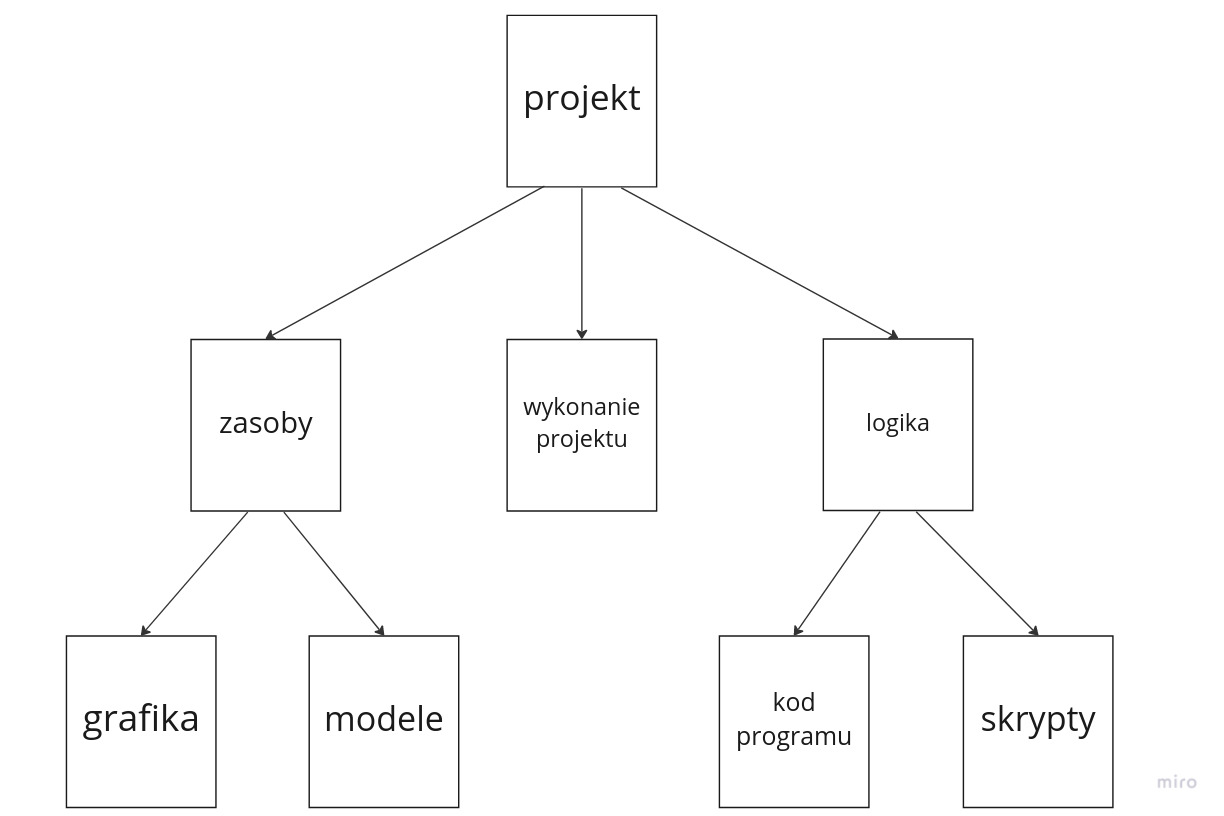
\includegraphics[scale=0.3,keepaspectratio]{images/diagrams/1 Project work categories.jpg}
        \end{center}


        \subsubsection{Modele i zasoby graficzne}
            Na zasoby wymagane do stworzenia projektu składać się będą modele trójwymiarowe oraz grafiki. Modele trójwymiarowe i tekstury zostaną użyte do stworzenia obiektów w wirtualnej scenie. Na grafiki składać będą się zdjęcia, ikony i inne obrazy wymagane w graficznym interfejsie użytkownika. Obie te grupy będą statycznymi zasobami które zostaną użyte w projekcie, a większość z nich trzeba będzie wykonać własnoręcznie.
            \\
        
        \subsubsection{Modele trójwymiarowe}
            Głównymi elmentami tworzącym scenę będą modele trójwymiarowe. Wszystko co będzie zbudowane w wirtualnej scenie będzie zbudowane z tych modeli trójwymiarowych. Każdy z nich będzie musiał zostać osobno ręcznie wymodelowany na podstawie zdjęć i rysunków poglądowych. Wszystkie z nich będą musiały zachowywać odpowiednie proporcje, względem przedmiotu który odwzorywują. Kolejnym ważnym aspektem jest jednolita skala modeli w projekcie, dzięki temu, nie trzeba będzie ręcznie dopasowywać rozmiaru każdego z modeli z kolei.
            \\
            
            Meble w scenie będą mogły zostać użyte jako pojedyncze wolnostojące meble, albo parę modułów mebli stawnowiące większą całość, przykładem może być zbudowa kuchni gdzie parę szefek stanowią większą całość. Podobną zasadę można zastosować w większej skali, do zbudowania ścian pomieszcenia. Zamiast modelować wszystkie ściany pomieszczenia jako jeden model, można wymodelować parę różnych wariantów ściany, a potem z nich złożyć każdy dowolny pokój.
            \\
            
            Wymodelowane będzie parę wariantów ścian. Oprócz zwykłej ściany, będą rówież warainty, posiadające miejsce na wstawienie drzwi, oraz wariant z miejscem na okna i parapet. Moduły ścian będą podzielone i zaprojektowane w taki sposób, że będzie można je rozciągać do wymaganej szerokości, tworząc pokój o dowolnych wymiarach i kształtach. Dla urozmaicenia ścian, okna będą wstawione we wnęki, w które opcjonalnie wstawić będzie można parapety. Dodatkową ozdobą ścian będą listwy przy podłodze oraz sztukaterie przy suficie. Oba te elementy będą łatwe w rozciągnięciu i dopasowaniu do ścian ze względu na swoją jednowymiarowość.
            \\
            
            Elementem urozmaicającym ściany są też grzejniki, które wstawione są zazwyczaj we wnękę pod parepetem okiennym. Ważne jest to aby również wymodelować rury, które w rzeczywistości doprowadzają ciepłą wodę do grzejnika. Grzejniki żeberkowe będą musiały zostać wykonane w różnych szerokościach gdyż nie można ich łatwo skalować. Bardziej nowoczesne grzejniki posiadającą pofalowaną powierzchnię są bardziej przyjazne skalowaniu modelu.
            \\
            
            Meble będą posiadały bardziej skomplikowane i szczegółowe modele trójwymiarowe, oraz posiadać będą swoją teksturę. Meble nie będą mogły być tak łatwo skalowane aby nie zabużyć ich proporcji. Ważnym aspektem jest nałożenie tekstury, która czasami będzie musiała zostać realistycznie nałożona na model, przykładem mogą być drewniane meble, które tworzone są w bardzo określony sposób. Zaburzenie tego przyzwyczajenia, będzie się podświadomie rzucało uytkownikowi w oczy.
            \\
            
            Niektóre meble są stworzone z więcej niż jedengo materiału, więc wymagane będzie nałożenie dwóch lub więcej różnych obrazów jako jedną teksturę. W pewnych przypadkach nie będzie to wystarczające, oraz wymagane będzie podzielenie jednego obiektu na więcej niż jeden model trójwymiarowy, żeby móc wykonać go z dwóch, lub więcej, różniących się od siebie materiałów. Przykładem może być okno, którego rama jest wykonana z tworzywa sztucznego, albo drewna, ale jego szyby są szklane, czyli półprzeźroczyste.
            \\
            
            Niektóre obiekty sceny, ze względu na użyte różne materiały, będą musiały być podzielone na parę osobnych części. W przypadku okien muszą posiadać one swoje klamki, które są wykonane z innego materiału. Podział jednego obiektu na mniejsze uprości proces modelowania poprzez ponowne użycie wcześniej użytych modeli. W tym przypadku, klamki w każdym wariancie okien, będą takie same, więc można oszczędzić czas używając osobno tych samych klamek dla wszystkich okien.
            \\
            
            Wnętrze posiadać będzie również inne elementy, które sprawią że pomieszczenie będzie wyglądać bardziej jak prawdziwy dom. Przewidywane są dywany i niektóre artykuły RTV/AGD. Dywan będzie prostą powierzchnią z teksturą dywanu i nałożoną na mapą wysokości. Ważnym elementem, sprawiające że pomieszczenie będzie wyglądać jak dom, są sprzęty domowe. Przykładem jest telewizor, który jest często centralną częścią salonu, dlatego również trzeba będzie wymodelować parę różnych modeli telewizora, w różnych rozmiarach. 
            \\
            
            Kolejnym elementem do wymodelowania są lampy i żyrandole. Na pierwszy rzut oka będą kolejnymi obiektami które będa uwiarygadniać całą scenę, ale ich ukrytą funkcją będzie również oświetlanie sceny, podczas nocy. Okna będą przepuszczały światło słońca za dnia, a w nocy lampy będą częściowo oświetlać scenę, aby można byłoby zobaczyć pokój i jego otoczenie w różnych warunkach oświetleniowych.
            \\
            
        \subsubsection{Grafiki i obrazy}
            Grafiki wymagane na potrzeby projektu
            \\
                
        
        \subsubsection{Logika programu}
        
        \subsubsection{Wykonanie projektu}
    
        
\section{Realizacja projektu}
    \subsection{Rozplanowanie projektu}
    
    
    \subsection{Rozplanowanie scen i pomieszczeń}
        Jednym z główych zadań wizualizacji jest prezentacja produktu w naturalnym dla niego otoczeniu, dlatego ważne jest aby zaprojektować pomieszczenia, które będą wyglądać lepiej dzięki powieszeniu paneli na ścianach. Celem tych paneli jest ozdobienie i przełamanie monotonii dużych pustych ścian danego pomieszczenia, dlatego prezentowane pomieszczenie powinno posiadać dużą pustą ścianę. Ściana nie musi być całkowicie wyeksponowana, przy niej mogą stać meble, ale nie powinny one być zbyt wysokie, dlatego panele pasowałyby również nad łóżkiem w sypialni. Pomieszczenie musi posiadać dużą nieprzerwaną ścianę, zazwyczaj salon jest największym pokojem w mieszkaniu, ale korytarze też mogą posiadać długie i monotonne powierzchnie.
        \\
        
        Zazwyczaj na zdjęciach wizualizacjach pokazany jest jeden wąski kadr przedstawiający produkt w swoim otoczeniu. Można by lepiej użyć medium interaktywne poprzez wyznaczenie paru interaktywych ścian w jednym pomieszczeniu lub mieszkaniu, pomiędzy którymi możnaby się przełączać. Każda z nich byłaby w trochę innym otoczeniu, symbolizujące inne pomieszczenie. Kamera zamiast przeskakiwać do osobnego pomieszczenia przesuwałaby się płynnie na kolejne miejsce i obracała kadr w kierunku nowej interaktywnej ściany. Wymaga to zaprojektowania mieszkania spcjalnie pod tym kątem.
        \\
        
        Zaprojektowanie pomieszczeń pozwoli na określenie ilości i umiejscowienia interaktywnych ścian pomieszczenia, rozplanowanie rozmieszczeń kamery oraz jej kadrowanie. Ważnym aspektem jest też rozplanowanie naturalnego i sztucznego oświetlenia w pomieszczeniu co odbywa się poprzez rozmieszczenie okien, lamp i żyrandoli. Po wstępnym zaprojektowaniu pomieszczeń, wiadoma będzie liczba i rodzaj mebli, które będa potrzebne do jego odtworzenia i umeblowania pomieszczenia za pomocą modeli trójwymiarowych. Dopiero wtedy można przejść do kolejnego punktu, którym jest wykonanie listy wymaganych modeli, oraz wymodelowanie ich. Dodatkowo, gotowy plan pomieszczenia ułatwi odwzorowanie go w silniku Unity3D.
        \\
        
        \subsubsection{Plany pomieszczeń}
        Poniżej przedstawione są plany pomieszczeń, które mogą znaleść się w projekcie. Rozplanowanie pomieszczenia pozwoli na określenie miejsc w do których będzie przenosić się kamera, oraz jaki kadr będzie ona obejmować. Na rysunku punkty oznaczają miejsca ustawienia wirtualnej kamery, a kolorowy trójkąt oznacza pole widzenia kamery, które na rysunku wynosi 60 stopni, co jest domyślnym ustawieniem kamery w Unity3D
        \\
        
        Pierwsze z nich jest fragmentem większego mieszania z aneksem kuchennym i osobnym pokojem. Dzięki jednej dużej przestrzeni w planie mieszkania, jedno pomieszczenie jest w stanie pokazać produkt w paru różniących się od siebie otoczeniach, w salonie, jadalni, kuchni i korytarzu. 
        \\
        \begin{center}
            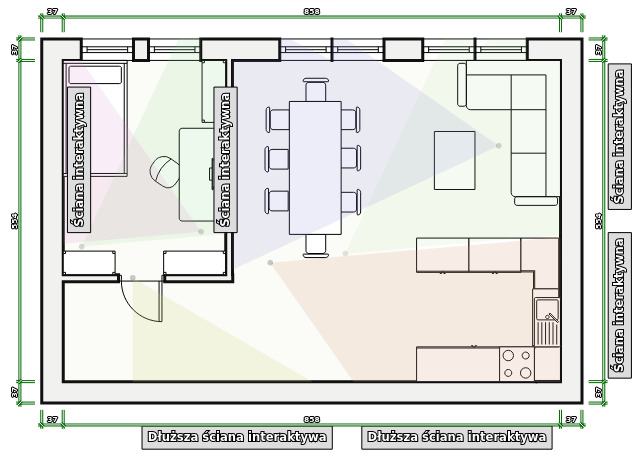
\includegraphics[scale=0.5]{images/diagrams/big_salon.jpeg}
            % big_salon.jpeg: 640x455 px, 72dpi, 22.58x16.05 cm, bb=0 0 640 455
        \end{center}
        
        
        Kolejny plan jest małą kawalerką. Modelowanie niewidocznych pomieszczeń i ich umeblowania nie jest wymagane, w tym przypadku łazienka nie będzie widoczna do wglądu, a jej drzwi będą zamknięte. Salon jest oświetlony naturlanym światłem, ale kuchnia wymaga dodatkowego, sztucznego światła.
        \\
        \begin{center}
            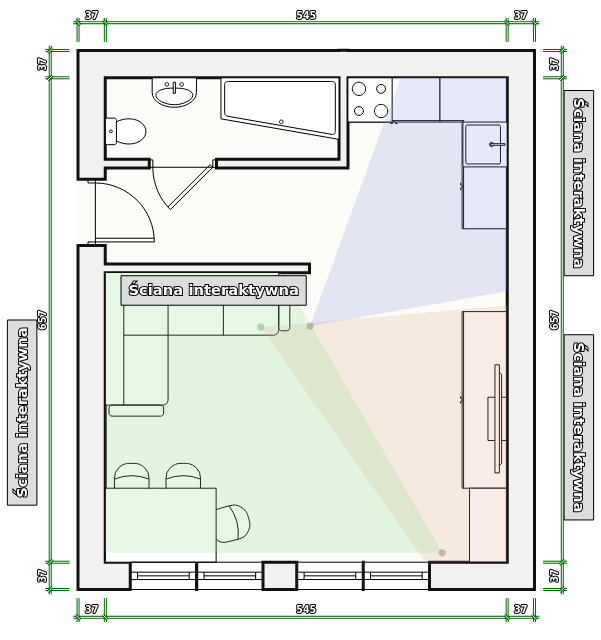
\includegraphics[scale=0.5]{images/diagrams/kawalerka.jpeg}
            % kawalerka.jpeg: 601x640 px, 72dpi, 21.20x22.58 cm, bb=0 0 601 640
        \end{center}

        Zależnie od ilości okien ilość światła naturalnego będzie większa lub mniejsza. W przypadku tego pokoju ilość światła słonecznego jest największa ze wszystkich przykładów. Otwartość przestrzeni pozwala na użycie mniejszej ilości sztucznych żródeł światła.
        \\
        \begin{center}
            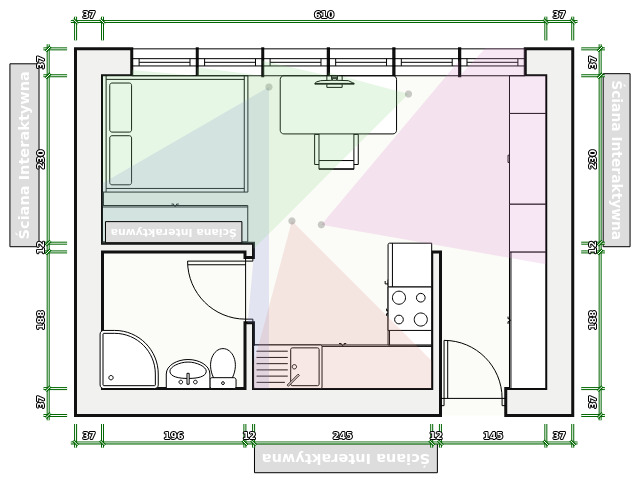
\includegraphics[scale=0.5]{images/diagrams/kawalerka2.jpeg}
            % kawalerka2.jpeg: 601x640 px, 72dpi, 21.20x22.58 cm, bb=0 0 601 640
        \end{center}
        
        
        Jest to dosyć małe i ciasne mieszkanie, może być wymagane zmienienie ustawień wirtualnej kamery, poprzez zwiększenie kąta jej widzenia. Mała ilość naturlego światła musi zostać zrekompensowana poprzez większą ilość sztucznego światła.
        \\
        \begin{center}
            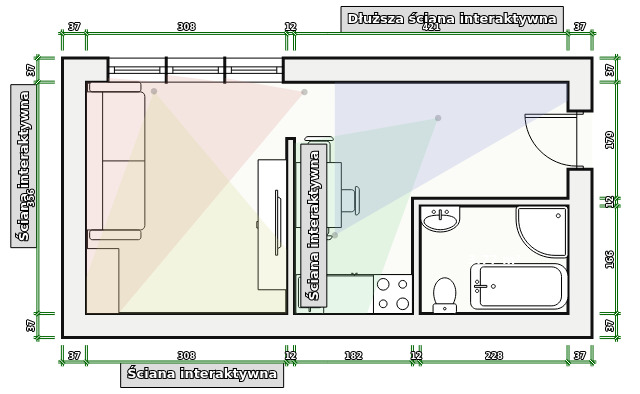
\includegraphics[scale=0.5]{images/diagrams/kawalerka3.jpeg}
            % kawalerka3.jpeg: 601x640 px, 72dpi, 21.20x22.58 cm, bb=0 0 601 640
        \end{center}
        
        
    \subsection{Modelowanie elementów 3d}
        Proste kształty i modele trójwymiarowe można modelować bez technicznych rysunków i planów, takimi modelami będą ściany, które będą prostymi powierzchniami, z opcjonalnymi wnękami i otworami na wstawienie okien lub drzwi. Jedyną rzeczą o której trzeba pamiętać jest zachowanie jednakowej skali oraz proporcji. Podłoga i sufit będzie jeszcze prostrza do wymodelowania, gdzyż będzie ona jedynie płaską powierzchnią. Posiadać ona będzie teksturę która urozmaici monotonną powierzchnię.    Bardziej wymagające do wymodelowania będą meble, które posiadają bardziej skomplikowane kształty, teksturę oraz materiały. 
        \\

        \subsubsection{Modelowanie ścian}
            Pierwszymymi elementami do wymodelowania będą części składające się na pomieszczenie: ściany, podłogi i sufity. Należy je zaprojektować i wymodelować w taki sposób aby możliwe byłoby proste ich rozciąganie, aby zmniejszyć ilośc modeli użytych w projekcie. Dodatkowo wydzielić można parę gotowych segmentów, z których można będzie zbudować większość pomieszczeń, będą nimi: pusta ściana, ściana z otworem na drzwi, ścina z otworem na okno, oraz ściana z wnęką pod grzejnik i otworem na okno. Wbrew pozorom z tych gotowych części będzie można złożyć większość podstawowych pomieszczeń. Ważne aby wszystkie modele w projekcie były wymodelowane w tej samej skali, a wymodelowane segmenty ścian powinny przestrzegać podstawowych zasad i wymiarów, którymi kierują się architekci podczas projektowania budnyków. Stworzenie niewymiarowych ścian burzyło by immersję użytkownika.
            \\
            
            <opisz proces modelowania ścian>
            \\
            
            Moduły ścian będa najprostrzymi do wymodelowania częściami ze względu na swoją prostą budowę. Będą one miały jednakowe wymiary: szerokość 1-go metra i wysokość 2,5 metra. Pusta ściana będzie jednolitą pionową powierzchnią o określonych wymiarach. Wariant z otworem na drzwi, posiadać będzie fragment ściany nad drzwiami, oraz ściany w które wstawiać będzie się drzwi. Ściana z otworem na okna będzie posiadać wariant uproszcony jedynie z otworem na okno na odpowiedniej wysokości, albo posaidać będzie również wnękę na grzejnik, pod otworem na wstawienie okna.
            \\
            
            Przed wyeksportowaniem modelu trzeba pamiętać o pewnych mniej oczywistych zawiłościach, jedną z nich jest sposób w jaki różne silniki graficzne interpretują modele. Domyślnie w programie blender każda ściana ma dwie strony, tą która jest widoczna, oraz druga która jest całkowicie nie widoczna, pozwala to na nie renderowanie niewidocznych ścian w projekcie. Program blender zawsze pokazuje każdą ścianę z obu stron, ale nie jest to prawdą dla silnika Unity3d, przez co niektóre ściany modelu mogą być nie widoczne z pewnych stron. Możliwe jest włączenie specjalnego trybu pokazującego które ściany będa widoczne oraz ustawienie ich w taki sposób, aby ściany były widoczne z odpowiedniej strony.
            \\
            
            Wykonane segmenty ścian są bardzo proste w swojej budowie i przezentują się następująco.
            \\
            <wstaw zdjęcie zegmentóœ ścian>
            \\
            
        \subsubsection{Modelowanie listw ściennych}
            Ozdobnymi częściami ścian będą listwy przypodłogowe oraz listwy przysufitowe. Oba przykłady listw mają dosyć proste do wymodelowania kształty. Są one jedynie przekrojem rozciągniętym w swojej długośći. Dokładny kształt przekroju listwy jest często przedstawiany w katalogu produktów, z uwagi na prostotę modelu jest to wystarczająco dokładna referencja. Z katalogu więc można skopiować przekrój listwy oraz wkleić go bezpośrednio do programu do modelowania jako zdjęcie referencyjne.
            \\
            
            Następnie trzeba zeskalować zdjęcie referencyjne do wymiarów zbliżonych do wynikowego modelu, w tej sytuacji bardzo pomaga prawidłowe ustawienie jednostek, oraz siatki w programie Blender. Dopomóc sobie można również ustawiając w pobliżu obiekt o ustalonych wymiarach, na przykład, sześcian o boku 10-ciu centymetrów. Skala i wymiary listwy i tak będą dostosowane podczas modelowania, aby wszystkie listwy miały podobne wymiary i tę samą skalę. 
            \\
            
            Najpierw trzeba ustawić odpowiednio punkt przyłożenia modelu, aby jego ustawienie było jednakowe z ustawieniem go w modelach ścian. Następnie można wymodelować przekrój listwy, odysowywując kolejne punkty wedle rysunku poglądowego. Powstały zarys przekoroju należy potem rozciągnąć go do końcowej długości listwy. W tym przypadku będzie to standardowa długość dla modułów ścian czyli 1. metr szerokości. Każda listwa posiadać będzie dwa warianty modelu, listwy przycięte prostopadle, oraz pod kątem 45-ciu stopni. Pozwoli to na tworzenie kątów i krawędzi ścian z idalnie schodzącymi się listwami.
            \\
            
            <wstaw rysunek>
            \\
            
            W taki sam sposób modelowane są listwy podsufitowe czasami nazywane sztukateriami. Różnicami będzie przesunięty punkt centralny modelu gdyż siatka będzie miała 1 metr a sufit będzie ustawiony na wysokości 2,5 metra. Kolejną różnicą będą dostępne wersje kolorystyczne z uwagi na różnice w materiałach zazwyczaj używanych do ich wykonania. Listwy przypodłogowe wykonywane są z drewna albo plastiku i mają albo teksturę drewna, albo jednolity kolor. Drewniane sztukaterie nie są już spotykane we współczesnych wnętrzach, ale były wykorzystywane w dawnych czasach kiedy ściany również zdobiono drewnianymi panelami. Dlatego sztukaterie nie będa posiadać tekstury, lecz jednolity zazwyczaj jasny kolor.
            \\
            
            
        \subsubsection{Modelowanie okien}
            Okna nie będą tak łatwo skalowalne jak ściany, dlatego będą wykonane w standardowym wriancie posującym do tworów na nie. By nie używać wszędzie tego samego modelu, trzeba będzie wykonać ich parę wariantów. Dostępne będzie pojedyncze okno, podwójne okno, oraz wysokie okno, które rozmairami i zastosowaniem przypomina przeszklone drzwi. Rama okna jest dosyś prosta do wymdelowania i można ją wymodelować na podstawie ogólnych wymiarów i zdjęć referencyjnych. Do wymodelowania klamki można użyć rysunków technicznych dostępnych na stronie producenta klamek do okien.
            \\
            
            Okno jest pierwszym modelem, który posiadać będzie więcej niż jeden materiał, lub teksturę. Podział jest dosyć prosty, gdzie osobne elementy okna wykonane są z innych materiałów. Rama okna jest wykonana z drewna, albo materiału o podobnym kolorze, szyba będzie przeźroczystą powierzchnią, a cała klamka wykonane będzie z metalicznego materiału o szorstkim wykończeniu. 
            \\
            
            Niestety nie jest możliwe bezpośrednie wyeksportowanie zawansowanych materiałów z programu blender do silnika Unity3D. Wyeksportować można jedynie tekstury, albo tekstury powstałe z tychże materiałów. Mimo tego, przydatne będzie na tym etapie przypisanie różnych materiałów do różnych części tego samego modelu, materiały będzie można zastąpić tymi pochodzącymi z silnika Unity3D. Na potrzeby tego projektu materiały silnika Unity3D są wystarczające.
            \\
            
            
        \subsubsection{Modelowanie mebli}
            Modelowanie mebli jest o wiele bardziej skomplikowane ze względu na ich bardziej złożone kształty. Jest jednak pewna metoda, która pozwala na proste i szybkie modelowanie modeli, z użyciem rysunków technicznych modelowanego obiektu. Polega ona na ustawieniu rysunków w przestrzeni trójwymiarowej oraz modelowaniu kolejnych części patrząc jednocześnie na więcej niż jeden rzut. W ten sposób stawiając punkt można sprawdzać poprawność jego umiejscowienia wielu osiach jednocześnie.
            \\
            
            Najpierw trzeba znaleźć rysunki techniczne, które przedstawiają modelowany obiekt z przodu, z boku oraz z góry. Czasami rysowane są dodatkowe rzuty, ale w większości przypadków nie są one niezbędne. Ważne jest, aby obiekt w każdym z narysowanych rzutów był narysowany w tej samej skali. By można było je ze sobą zestawić w przestrzeni trójwymiarowej.
            \\
            
            Niektóre firmy meblowe, w ramach marketingu i promocji swoich mebli, udostępniają za darmo modele trójwymiarowe swoich mebli, zdjęcia oraz ich rysunki techniczne. Projekt tworzony na potrzeby tej pracy inżynierskiej nie będzie wykorzystywany komercyjnie, więc można użyć w nim własnoręcznie wykonanych modeli opierających się na rysunkach udostępnionych do publicznego użytku. Czasami nawet udostępniane są gotowe oteksturowane modele trójwymiarowe mebli z zastrzeżeniem nie używania  go w projektach komercyjnych. Jedyną różnicą będzie fakt wykonania tychże modeli od podstaw.
            \\
            
            Proces modelwoania skoplikowanych modeli, zaczynamy od zaimportowania jego rysunków technicznych do programu Blender. Kopiujemy go tylerazy, ile rzutów jest narysowanych na rysunku. Każdy z rysunków ustawiamy w taki sposób aby był widoczyny z innej strony: front, bok, góra. Potem tworzymy podstawowy obiekt, kostkę która pomoże zestawić je ze sobą w przestrzeni trójwymiarowej. Kostkę skalujemy do odpowiednich wymiarów, zazwyczaj są to wymiary zakreślające cały obrys przedmiotu, z każdej widocznej perspektywy. Przesuwamy pojedynczo rysunki w jednej płaszczyźnie jednocześnie, aż do czasu kiedy przedmiot w każdym rzucie, mieści się w obrębie kostki.
            \\
            
            Kolejnym ułatwieniem medium cyfrowego jest to, że nie jeżeli modelowany przedmiot jest symetryczny, to nie trzeba modelować go w całości. Im więcej osi symetrii ma model tym mniejszą część należy modelować. Krzesło mając jedną oś symetri można podzielić na dwie połowy, stół natomiast posiada dwie osie symetrii, więc wystarczy wymodelować jego ćwiartkę. W przypadku krzesła wystarczy wymodelować jego połowę, a potem użyć modyfikatora, który stworzy drugą połowę modelu w odbiciu lustrzanym, pamiętać należy, że odbicie to tworzone jest względem punktu centralnego modelu.
            \\
            
            \subsubsection*{Modelowanie krzesła}
            Teraz można zacząć proces modelowania. Zacząć można od jednego z podstawowych kształtów i powoli dodawać kolejne punkty, linie i ściany. Wielkim ułatwieniem jest fakt, że stawiając nawet jeden kolejny punkt, można sprawdzić poprawność jego położenia w paru rzutach jednocześnie, zamiast przełączać się po kolei pomiędzy nimi.
            \\
            
            \begin{center}
            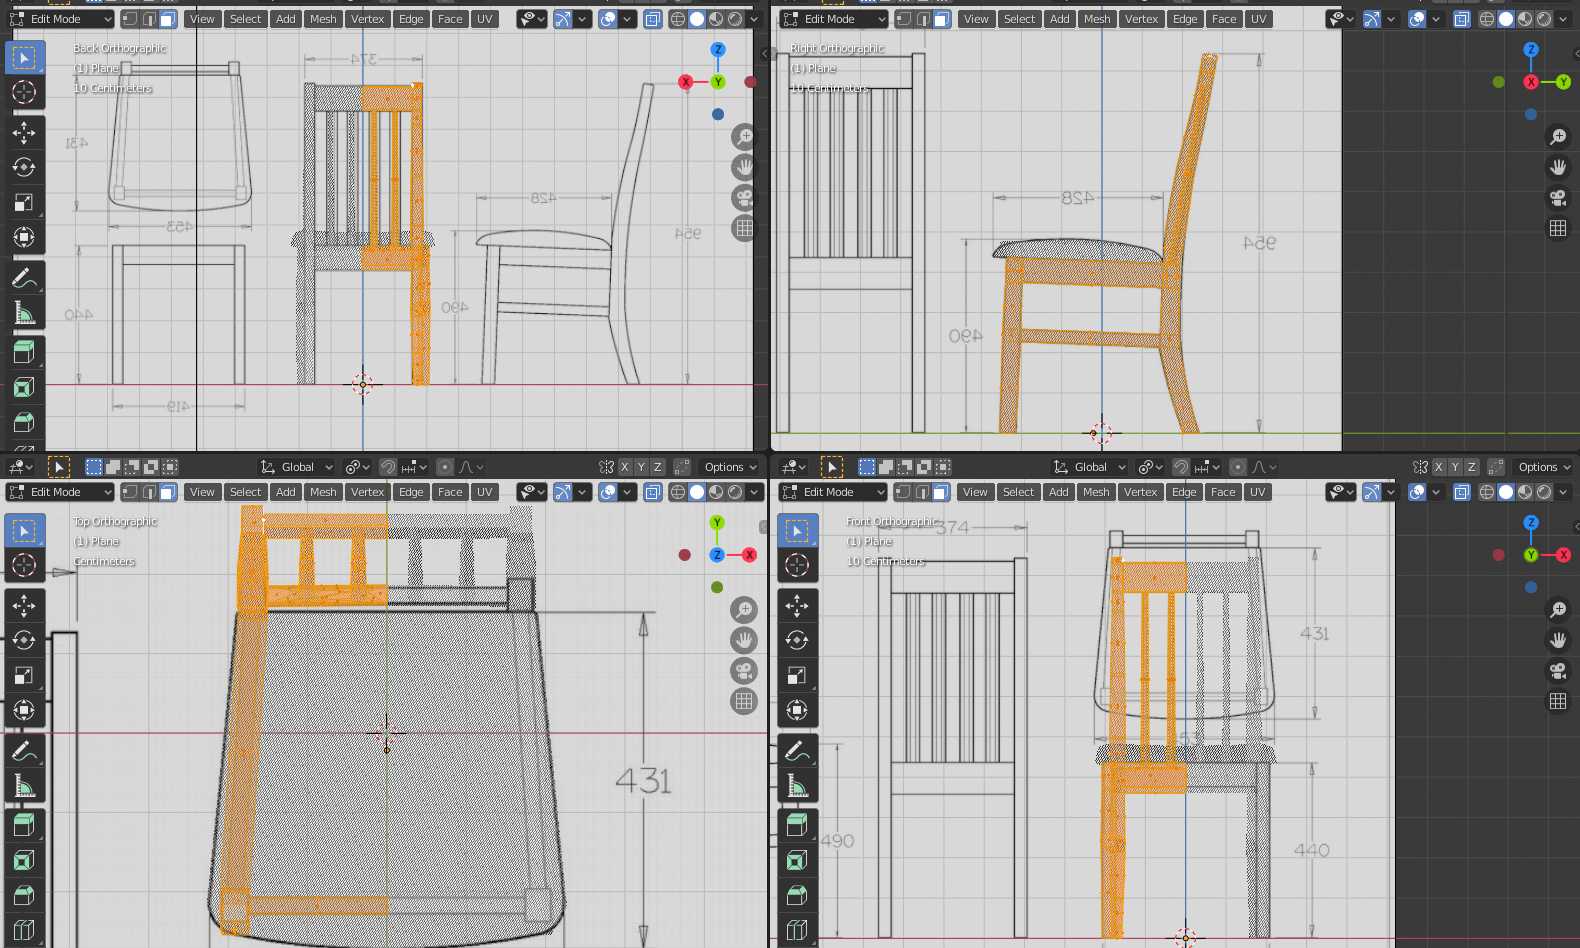
\includegraphics[scale=0.25,keepaspectratio=true]{images/screenshots/work/5-modelowanie-mebli_004.png}
            % 5-modelowanie-mebli_004.png: 1580x948 px, 72dpi, 55.74x33.44 cm, bb=0 0 1580 948
            \end{center}
            
            Rama krzesła modelowana jest najpierw jako dwuwymiarowy kształt. Najpierw tworzony jest przekrój nogi krzesła, potem odchodzace od niego poprzeczki, następnie można rozciągnąć dwuwymairowy obiekt do trójwymiarowego tworząc zalążek ramy siedziska.
            \\
            
            Za wczasu w miejscach zamontowania nóg krzesła powstawiane zostały kwadraty, będące jednocześnie przekrojami każdej z nóg krzesła. Kwadraty będą podstawą do stworzenia kwadratowych nóg krzesła. Tworzenie długich kształtów jest dosyć proste, wystarczy zaznaczyć ścianę która jest spodem nogi, oraz rozciągnąć ją do wybranej długości. Nogę rozciągamy do momentu montowania poprzeczki pomiędzy tylną a przednią noga krzesła. Podczas dostawiania każdego kolejnego przedłużenia na osobnym widoku sprawdzamy jego długość, a na innym jego dokładne położenie w innych osiach. W podobny sposób modelujemy oparcie krzesła, będące przedłużeniem tylnych nóg. WYstarczy powstawiać proste okrągłe szczebelki kończąc krzesło.
            \\
            
    \subsection{Części projektu}
        \subsubsection{Logika i schemat działania}
        \subsubsection{Interfejs użytkownika}
        \subsubsection{Widok pomieszczenia}
        \subsubsection{Hierarchia i diagramy klas}
        \subsubsection{Osadzenie programu wynikowego na stronie internetowej}



\section{Wnioski}


\newpage
\section{Literatura}

\newpage
\section{Załączniki}



\end{document} % This is the end of the document

